\subsection{Difference-in-differences}
We start by presenting results for the data with imputed ethnicity (adjusted with full matrix correction from equation \ref{eq:full_matrix_adj} and date of arrest since we consider them to be the most credible. However, we also consider how the results change if do not impute or apply different adjustment further in the paper. 

 The estimated coefficients  $\beta_k$ from the dynamic difference-in-differences model (\ref{eq:dynamic_did}) are plotted in the figure \ref{fig:did_effets}. 
 We can draw several conclusions from the results. 
 First, the coefficients from 1933 to 1938 are not significantly different from zero which implies that hostility between Germany and the Soviet Union in this period does not seem to impact the repressions of Germans contrary to the theoretical predictions. Second, the political arrests of Germans start to rise in 1939 which is surprising given that  Molotov-Ribbentrop pact guaranteeing neutrality Germany and the USSR was signed that year. The repressions then peak  with start of the war at 1941 (although there is some slight drop from 1942 to 1944). Finally, the effects of war on the repressions appear to be highly persistent as there is no decline in the arrests after 1945. 
 %There even
 
 \begin{figure}[h]
\centering
\caption{Estimates of $\beta_k$ from the Specification \ref{eq:dynamic_did}}
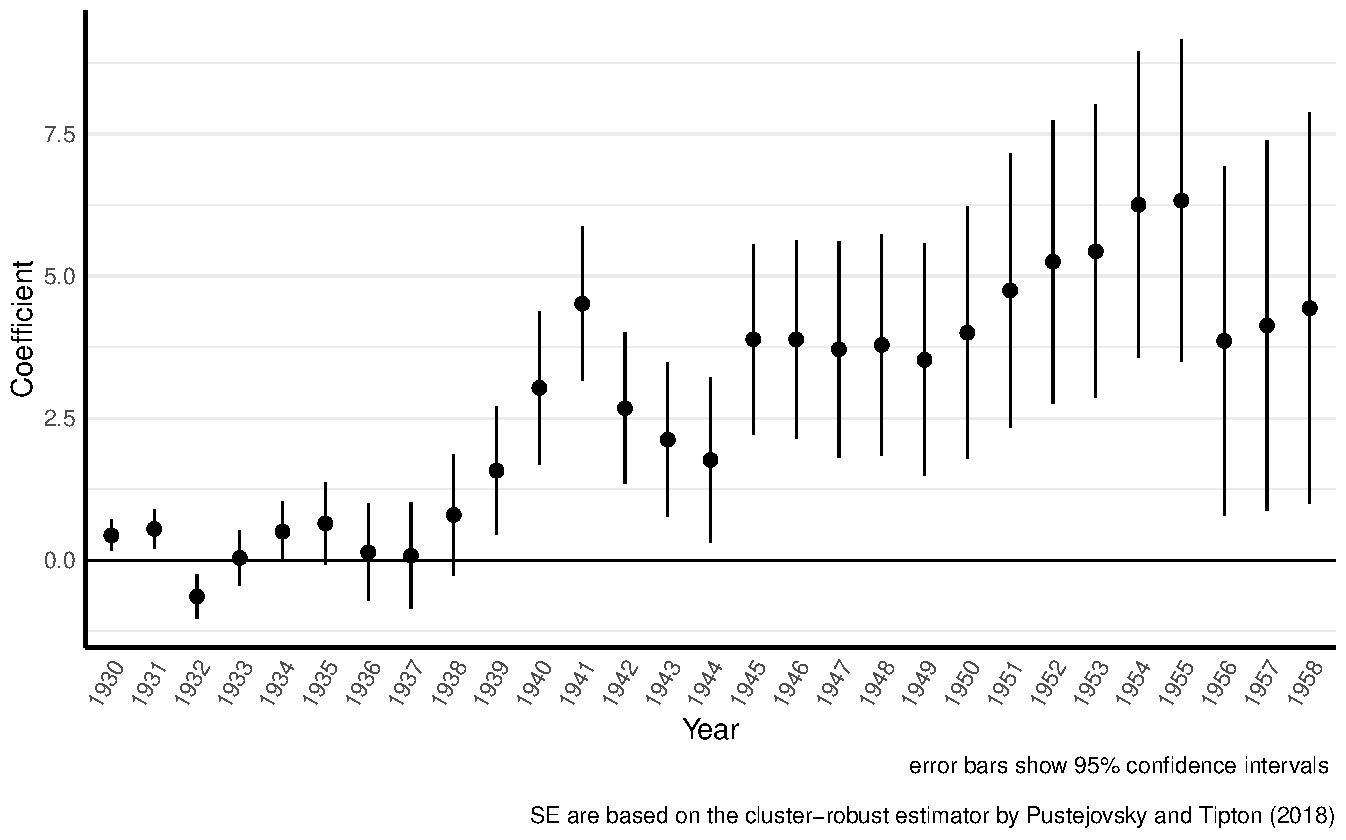
\includegraphics[width=\textwidth]{plots/effects/ethnicity_imputation/annual/point_range_robust_cr2_date_imp_full_years.pdf}
\begin{minipage}{0.92\textwidth}
%\includegraphics[width=\linewidth]{Gaus.pdf}
%\rule{\linewidth}{10em}
\footnotesize
\emph{Notes:} Ethnicity and date of arrest were imputed.  Full matrix adjustment was applied on ethnic group imputations. All 38 ethnic groups are included.  Standard errors are based on cluster robust estimator by \citet{pustejovsky_small-sample_2018}. Error bars show 95\% confidence intervals. 
\end{minipage}
\label{fig:did_effets}
\end{figure}

 
 The results from the time window specification (equation \ref{eq:simple_did}) shown in the figure \ref{fig:did_effets_time_window} tell the same story.  The coefficients in the model imply that in the period of Molotov-Ribbentrop pact and war, the arrests of Germans were about 2\% higher than the arrest other ethnic groups. Surprisingly, the estimated effect in the post-war period is higher still at  3.6\%.
 
 \begin{figure}[h]
\centering
\caption{Estimated Coefficients for Specified Time Windows from the Specification \ref{eq:simple_did}}
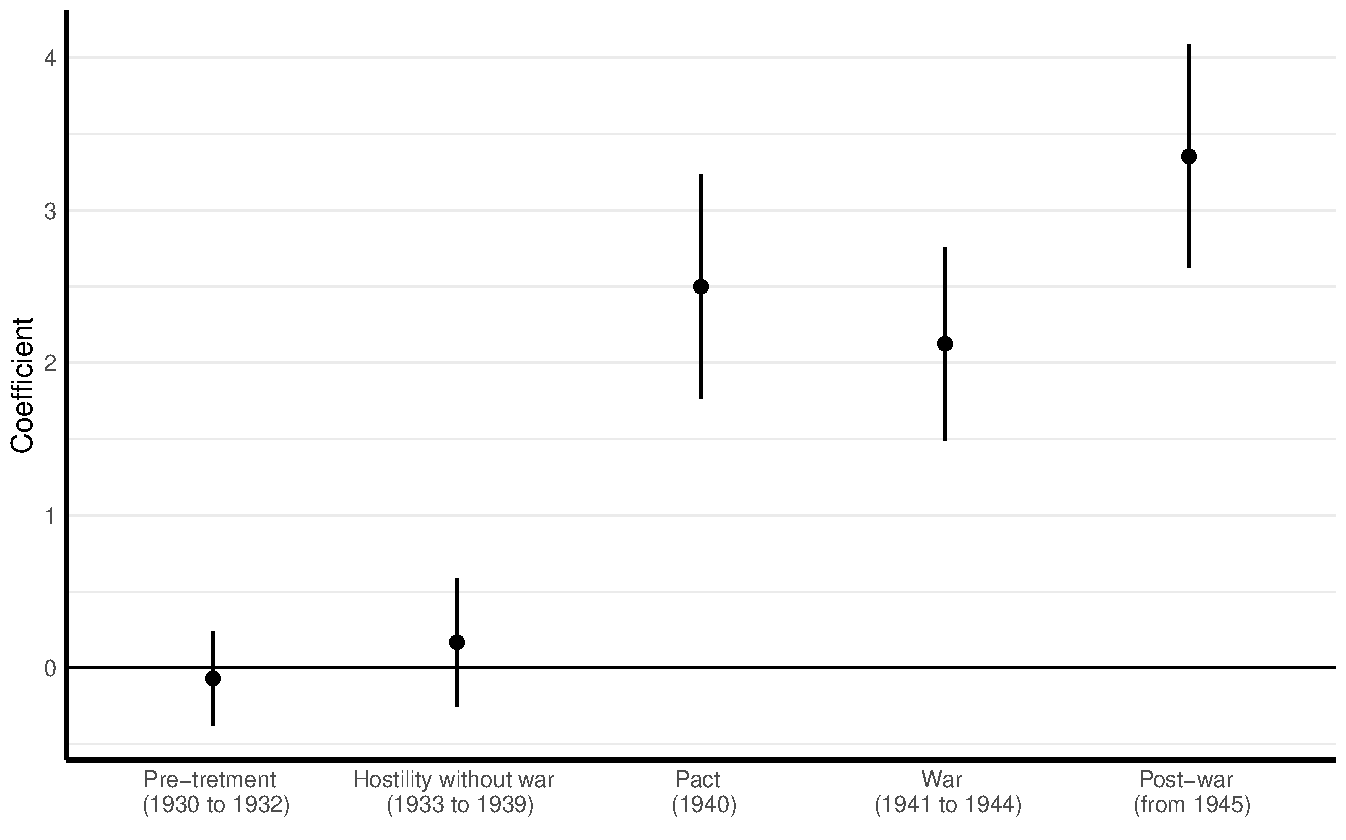
\includegraphics[width=\textwidth]{plots/effects/ethnicity_imputation/annual/time_window_pre_treatment_date_imp.pdf}
\begin{minipage}{0.92\textwidth}
%\includegraphics[width=\linewidth]{Gaus.pdf}
%\rule{\linewidth}{10em}
\footnotesize
\emph{Notes:} Ethnicity and date of arrest were imputed.  Full matrix adjustment was applied on ethnic group imputations. All 38 ethnic groups are included. Standard errors are based on cluster robust estimator by \citet{pustejovsky_small-sample_2018}. Error bars show 95\% confidence intervals. 
\end{minipage}
\label{fig:did_effets_time_window}
\end{figure}
 
However, the pre-1933 coefficients in the figure \ref{fig:did_effets} give us some reason to doubt the
validity of our model. Even though they are small in size relative to the post-1939 coefficient, they are all  significantly different from 0 at 5\% level.
%and others are very close to being significant. 
This provide some evidence that the pre-treatment trends for German minority were not parallel with trends for other ethnic groups. We can thus suspect that the post-treatment trends were not parallel either which
would violate the basic identifying assumption of
difference-in-differences.
%The deviations from parallel trends in the pre-treatment period are relatively small possibly indicating that the bias might not be as large. 
We address this problem by applying the synthetic control method in the next section. 
%Bearing in mind these potential problems, we proceed 
 
Another potential issue is that some ethnic groups changed their treatment status in this period in various complicated ways. For example, Poland was invaded by the USSR and Germany but it took  only about month until the Polish forces were defeated. The Baltic states were annexed and incorporated into the Soviet Union in June 1940 only to be invaded by Germany year later. 
It is difficult to decide what treatment status should we assign in these cases. 
Moreover, given the scale and complexity of World War 2, the USSR experienced  some kind of change in geopolitical relations with almost every country in its neighborhood.  

To address this issue, we exclude every ethnicity which constituted a core group in some independent state in the interwar period from the dataset (except for Germans, of course) and reestimate the model. This criterion removes 10 ethnic groups from the dataset. The full list of them is provided in the table \ref{tab:sc_predictors}. The results of the dynamic difference-in-differences are plotted in the figure \ref{fig:did_effets_no_ind_countries} in the appendix. The estimated coefficients change  very little compared to the results with all ethnic groups included, only confidence intervals appear slightly wider since we have fewer observations. Therefore our previous results are maintained. 

In the section \ref{subsec:robust_checks}, we perform several additional robustness checks to further asses the sensitivity of our findings. In particular, we refit the models for different ethnicity-specific time-trends and imputation adjustments. 

%Bearing in mind these potential problems, we continue by considering different sets of control groups to better understand what drives the results. 
 
 %The coefficients between the years 1933 and 1939 (when the relations between Germany and Soviet Union were hostile) mostly range  between 1 and 3 and all except one are statistically significant at 5\% level. The rise of Nazism thus based on these estimated increased the arrests of Germans by the NKVD in the USSR by about 2\%.  

%However, the pre-1933 coefficients give us some reason to doubt the
%validity of our model. Three of them are significantly different from 0 at 5\% level and others are very close to being significant. 
%This provide some evidence that the pre-treatment trends for German minority were not parallel with trends for other minorities. We can thus suspect that the post-treatment trends were not parallel either which would violate the basic identifying assumption of difference-in-differences. To address this concern, we apply the synthetic control method which can be valid even in the absence of  parallel trends. 
%We can see that all coefficients for years 1930 to 1932 are statistically insignificant which means that the pre-treatment trends in arrests of German minority were likely parallel to the pre-treatment trends of other minorities which gives us greater  confidence in the validity of our identification strategy. 

%The coefficients on all other years are insignificant as well. Only for 1934 (one year lag) is the estimate  significant at 10\% level ($p$-value of 0.08). Since this not reaches even the traditional 5\% significance threshold we are inclined to not reject the null hypothesis or at least to conclude that evidence in favor of the alternative hypothesis (more repressions of Germans due to rise of Hitler) is quite weak.  Furthermore, as we show below the alternative specifications do not increase the significance of the coefficients.






%We perform several robustness checks to asses sensitivity of the results to different specifications. First, in our main model (column (1) of table \ref{dif_table}), we included all observations in years 1923 to 1958. But the relationship between Germany and Soviet Union were somewhat more complicated after the World War II. We thus re-estimate the model with only the data from 1923 to 1945. The results (in column (2)) change only little and does not alter our previous conclusions. Second, when we omit the ethnicity specific linear time trends in column (3), we see again that the coefficients are very similar to the original model. Finally, we estimate a specification with number of arrests as a dependent variable (without logarithmic transformation). We can see that this model (shown in column (4)) fits the data rather poorly with  $R^2$ only of 0.428 (compared to 0.890 in the logarithmic specification). 

%We perform several robustness checks to asses sensitivity of the results to different specifications. First, in our main model (column (1) of table \ref{dif_table}), we included all observations in years 1923 to 1958. But the relationship between Germany and Soviet Union were somewhat more complicated after the World War II. We thus re-estimate the model with only the data from 1923 to 1945. The results (in column (2)) change only little and does not alter our previous conclusions. Second, when we omit the ethnicity specific linear time trends in column (3), we see again that the coefficients are very similar to the original model. Finally, we estimate a specification with number of arrests as a dependent variable (without logarithmic transformation). We can see that this model (shown in column (4)) fits the data rather poorly with  $R^2$ only of 0.428 (compared to 0.890 in the logarithmic specification). 


\subsection{Synthetic Control Method}
We implemented the synthetic control method in R  using the MSCMT package \citep{becker_fast_2018}.
Our outcome variable is again $\log\left(1 + \text{arrests}\right)$.
As in the difference-in-difference, we include all 38 ethnic groups and we impute missing date of arrest and ethnicity (which we adjust using the full-matrix correction).
In our baseline model, the  outcomes for all pre-treatment years (1921-1932)  were included  as predictors. 
This approach has been widely used in the literature \citep{billmeier_assessing_2013, cavallo_catastrophic_2013, bohn_did_2014} and in contrast to other methods (such as using only mean of pre-treatment outcomes) it  has the advantage  of reducing opportunities of specification search  \citep{ferman_cherry_2018}. 
We also include three time-invariant covariates that might potentially be predictive of post-1933 repressions: total population of the ethnic group in the USSR, its urbanization rate (both taken from the 1926 Soviet census), and linguistic similarity to Russian. 
However, including all pre-treatment outcomes as predictors  renders  other  covariates unimportant in the optimization procedure \citep{kaul_synthetic_2018}. On the other hand, \citet{botosaru_role_nodate} argue that if there is a long set of pre-treatment outcomes (which is our case) then a perfect balance on covariates should not be required.
Since there is no clear consensus in the literature, we apply both methods and show the synthetic control method with mean of the pre-treatment outcome as predictor in section \ref{subsec:robust_checks} as a robustness check in addition to our baseline specification with  all pre-treatment outcomes as predictors that we present below. 

% Taken together, our results show that, while there may be advantages in balancing on covariates to construct the SC estimator, a perfect balance on covariates should not be required for the SC method, as long as there is a perfect balance on a long set of pre-treatment outcomes. O


The calculated optimal weights $W$ of ethnic groups in the synthetic German minority are provided in the table \ref{tab:sc_weights} (ethnic groups with zero weight are not shown). The highest contribution in the synthetic German minority have Russians, Greeks and Finns with weights 0.36, 0.28, and 0.17 respectively.  Lithuanians, the Khakas, Yakuts, and Bulgarians  are also represented in the synthetic control although only with  weights smaller than 0.08. 
\begin{table}[t]

\caption{\label{tab:sc_weights}Synthetic German minority weights}
\centering
\begin{tabular}{lr}
\toprule
Ethnic group & \$W\$-Weight\\
\midrule
Greek & 0.32\\
Kabardian & 0.09\\
Chuvash & 0.08\\
Moldovan & 0.07\\
Belorussian & 0.06\\
Polish & 0.06\\
Finnish & 0.06\\
Altai & 0.04\\
Armenian & 0.04\\
Georgian & 0.03\\
Ossetian & 0.02\\
Chechen & 0.02\\
Kazakh & 0.02\\
Bashkir & 0.02\\
Jewish & 0.02\\
Ukrainian & 0.01\\
Bulgarian & 0.01\\
Latvian & 0.01\\
Chinese & 0.00\\
\bottomrule
\end{tabular}
\end{table}

%The balance of covaria
%\begin{table}[!h]

\caption{\label{tab:sc_predictor_means}Pre-treatment Predictor Means}
\centering
\begin{threeparttable}
\begin{tabular}{lrrr}
\toprule
\multicolumn{1}{c}{ } & \multicolumn{2}{c}{German minority} \\
\cmidrule(l{2pt}r{2pt}){2-3}
Variable & Actual & Synthetic & Mean of all 38 ethnicities\\
\midrule
Log(1 + arrests) & 5.59 & 5.59 & 3.65\\
Total population & 1 238 549.00 & 28 292 179.83 & 3 681 250.42\\
Urbanization rate & 14.92 & 20.96 & 17.84\\
Ling. similarity to Russian & 1.00 & 2.29 & 0.76\\
\bottomrule
\end{tabular}
\begin{tablenotes}
\item \textit{Note: } 
\item Log(1 + arrests) is averaged over the pre-treatment period (1921-1932). All other predictor are time-invariant. Total population and urbanization rate are taken from 1926 Soviet census.
\end{tablenotes}
\end{threeparttable}
\end{table}


Figure \ref{fig:sc_comp_plot} shows the  arrests of the German minority and its synthetic control.
The synthetic control fits the actual pre-treatment values reasonably well. 
In the post-treatment period, both time series follow similar general trends (rise in 1937-1938 and decline after 1945). 
However up until 1955, the actual arrests of Germans are consistently higher than the predictions of  synthetic control. %We can get more detailed picture in 
We can infer the estimated effect size in the post-1933 period  from 
the figure  \ref{fig:sc_placebo_gaps_all} which shows the difference between the actual arrest and their synthetic counterparts for each year (on $\log(1 + x)$ scale). 

 \begin{figure}[h]
\centering
\caption{Comparison plot}
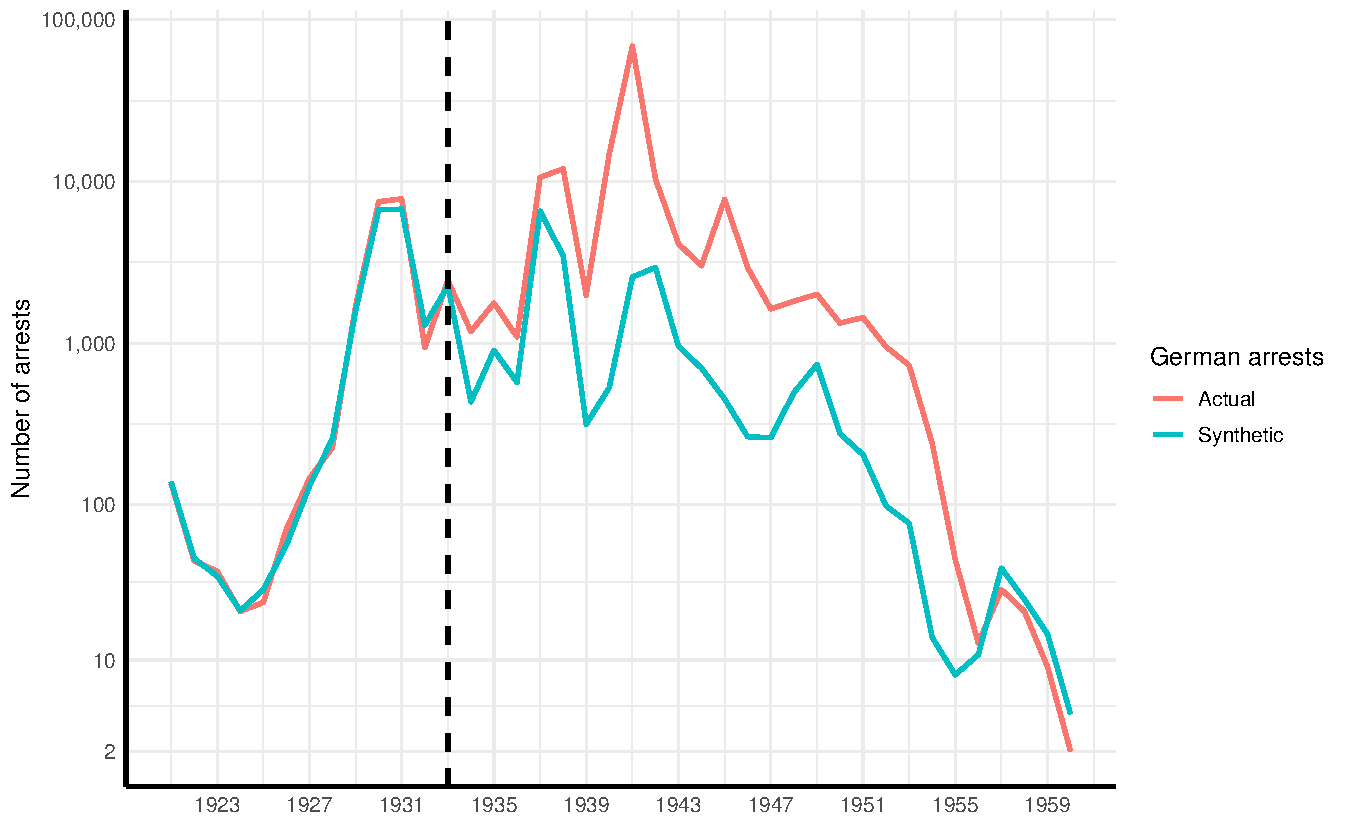
\includegraphics[width=\textwidth]{plots/synthetic_control/ethnicity_imputation/annual/comparison_plot_scaled.pdf}
\begin{minipage}{0.92\textwidth}
%\includegraphics[width=\linewidth]{Gaus.pdf}
%\rule{\linewidth}{10em}
\footnotesize
\emph{Notes:} The values on y-axis are shown on $\log\left(1 + y\right)$ scale.  Ethnicity and date of arrest were imputed.  Full matrix adjustment was applied on ethnic group imputations. All 38 ethnic groups are included. 
\end{minipage}
\label{fig:sc_comp_plot}
\end{figure}


From 1933 to 1939, this gap is close to 1. For the period from 1941 to 1955, the estimated effect is higher but also more volatile oscillating between 1 and 3 corresponding to 1 to 3\% increase in arrests of Germans in that period.  After 1955, the gap shrinks to zero. 
The results are similar to difference-in-differences in the overall trends. Nevertheless, the estimated effects by the  the synthetic control  are slightly smaller than the their difference-in-differences equivalents.  

%As we metioned in the section
We estimate significance of our results with placebo tests by applying the same procedure to every ethnic group in the dataset. The differences between the actual values and the respective synthetic control for every placebo ethnicity are plotted in grey in the figure \ref{fig:sc_placebo_gaps_all}. Even in comparison with the placebo tests, 
the estimated effect for German ethnicity  still appears relatively large for the period from 1939 to 1955 although for years 1933-1938 the effect for Germans seems within the standard range of the placebo gaps.

However, the figure \ref{fig:sc_placebo_gaps_all} also shows that for some ethnic groups the pre-treatment gaps are large too.
 For example, the gap for Russians stays above 2.5 for the whole pre-1933 period. 
 This indicates that synthetic control of these ethnic groups does not capture the actual pre-treatment trends well. 
 %In other words, no linear combination of ethnic group cannot 
 As we explained in the subsection \ref{subsec:sc_methodology}, the placebo synthetic contros  with with substantially  worse pre-treatment then the treated unit should not be 
used in estimating significance of the treatment effect. 
%are not very helpful for
%for estimating rareness of an effect for a treated unit with a good pre-treatment fit. 
We thus  exclude the placebo ethnicities whose pre-treatment mean squared prediction error (MSPE) is 20 times higher than the same measure for German minority. Even though this is relatively lenient cutoff, it removes x ethnic groups that does not meet the criterion. 
The resulting plot is shown in the figure \ref{fig:sc_placebo_gaps_all_20_times}. The post-1933 gaps in German arrests now stand out more clearly and even the gap for the years 1933-1938 now appears relatively significant.  
%They thus recommend excluding excluding placebo groups with substantially higher pre-treatment mean squared prediction error  (MSPE)

%Following \citet{abadie_synthetic_2010}  we therefore exclude ethnic groups whose pre-treatment MSPE is 5 times higher then the same measure for German minority. This removes 4 ethnic groups with the worst pre-treatment fit. The resulting plot is shown in the figure \ref{fig:sc_placebo_gaps_all_20_times}. The post-1933 gaps in German arrests now stand out more clearly. 


%The trends start to diverge in the second quarter of 1933 with the actual arrests of Germans holding steady but decreasing for synthetic control. 
%The gap between the trends for the actual German minority and its synthetic control (shown in figure \ref{fig:sc_placebo_gaps_all}) keeps within the range of 1.25 to 2.5 for most of the post-1933 period. This implies that the rise of Hitler led to about  2\% increase in the arrests of Germans by the NKVD  in the period from 1933 to 1939. This is very similar to the estimates obtained using difference-in-differences. 
%The figure shows increase between 1937 and 1939 (the period of the Great Terror).  




%\subsubsection{Inference}
%The estimated  gaps between the synthetic control and the actual data for every ethnic group is shown in figure \ref{fig:sc_placebo_gaps}. 

%are not very helpful for
%for estimating rareness of large  post-treatment gap for a treatment with a good pre-treatment fit. They thus recommend excluding excluding placebo groups with substantially higher pre-treatment mean squared prediction error  (MSPE)
%(the average of squared differences between the value of the outcome for synthetic and actual) 
%relatively to the treated group. 
%In our case the pre-treatment MSPE of the German minority is fairly small (0.52). 
%If we exclude minorities with the pre-treatment MSPE
%If we choose the cutoff for exclusion as the MSPE 

%Morever, the pre-treatment MSPE is quite small (0.52) which means that the synthetic German minority captures the actual pre-treatment trends relatively well. However, the pre-treatment MSPE of a few minorities is much larger indicating that no combination of donor ethnic groups fits well their time series. As \citet{abadie_synthetic_2010} note,  if there is poor fit of the synthetic control to the actual trends in the pre-treatment period then its post-treatment gap does not provide good comparison to the well fit ethnic groups. 
%large post-treatment gap would not indicate the presence of an effect but  
%Following \citet{abadie_synthetic_2010}  we therefore exclude ethnic groups whose pre-treatment MSPE is 5 times higher then the same measure for German minority. This removes 4 ethnic groups with the worst pre-treatment fit. The resulting plot is shown in the figure \ref{fig:sc_placebo_gaps_all_5_times}. The post-1933 gaps in German arrests now stand out more clearly. 

\begin{figure}[hbtp] 
\caption{Gaps between synthetic control and actual values for placebo tests}
\begin{subfigure}{\textwidth}
\caption{All ethnic groups}
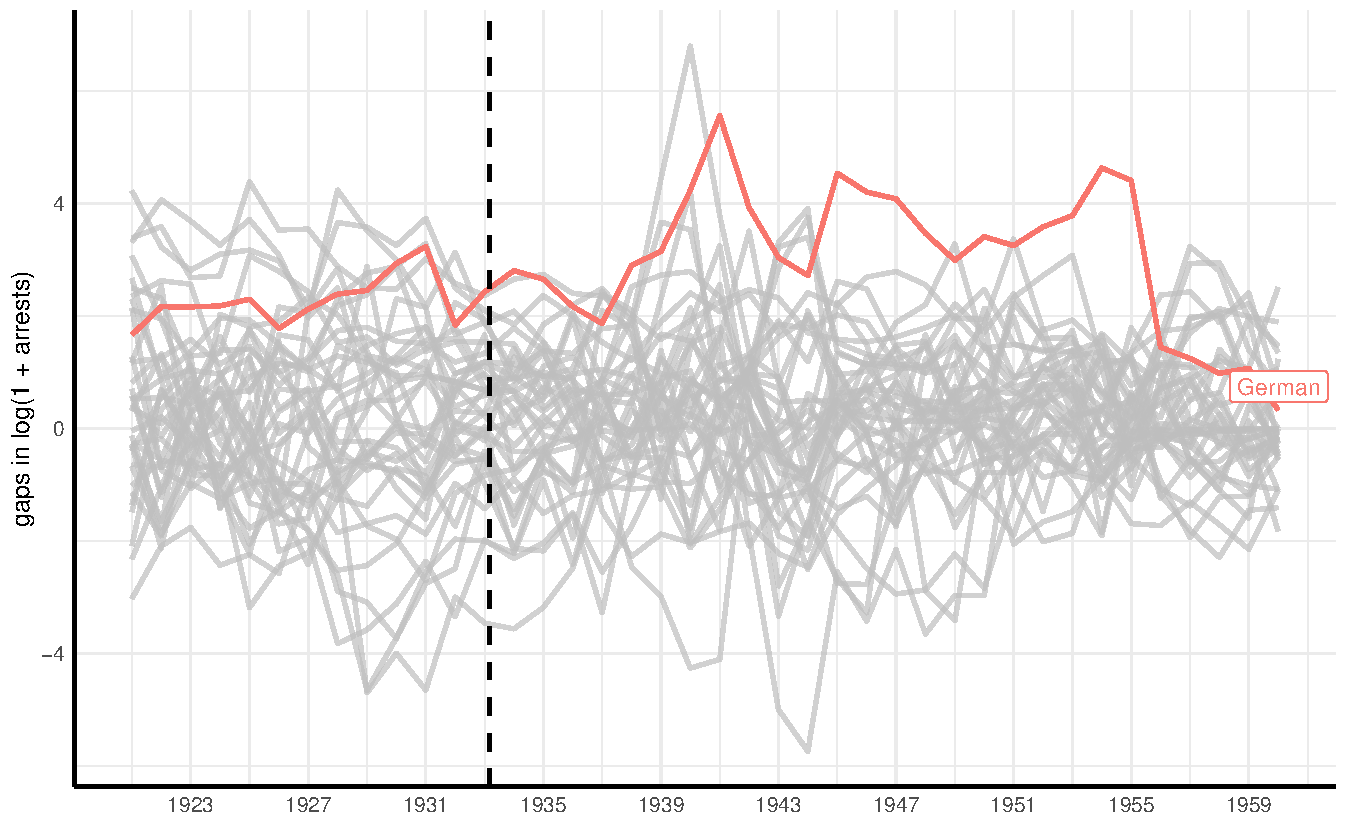
\includegraphics[width=0.9\linewidth]{plots/synthetic_control/ethnicity_imputation/annual/placebo_highlight_all_imp_date.pdf}
\label{fig:sc_placebo_gaps_all}
\end{subfigure}
\begin{subfigure}{\textwidth}
\caption{Ethnicities with pre-treatment MSPE higher than 20 times the MSPE of Germans excluded}
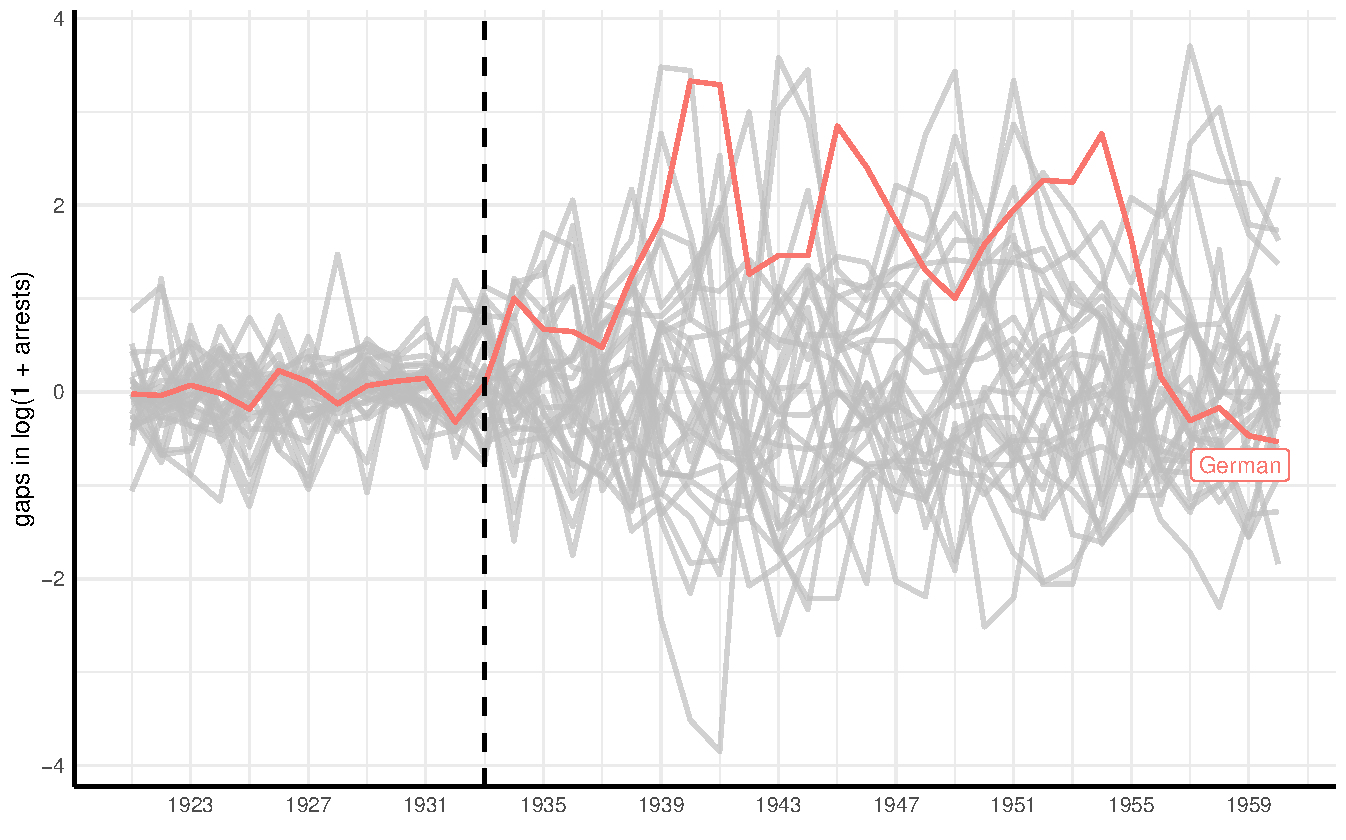
\includegraphics[width=0.9\linewidth]{plots/synthetic_control/ethnicity_imputation/annual/placebo_highlight_mspe_20lower_imp_date.pdf}
%Ethnic groups with pre-treatment MSPE higher than 5 times the MSPE of Germany excluded
\label{fig:sc_placebo_gaps_all_20_times}
\end{subfigure}
\label{fig:sc_placebo_gaps}
\end{figure}

Nevertheless, our preferred approach for assessing uncertainty in results that avoids  choice of any arbitrary level of the pre-treatment MSPE cutoff for the exclusion of poorly fit  placebos
is to compare the ratios of  post/pre-treatment MSPE. 
The values of these ratios for all ethnic groups are displayed in the figure \ref{fig:sc_mspe_ratios_all} for the whole post-treatment period. The MSPE ratio for the German minority is by far the highest. The probability of German minority having the highest ratio of all under the null hypothesis of zero treatment effect is 1/38 ($\approx 0.026$). 
In the figure \ref{fig:sc_mspe_ratios_until_1939}, we also provided the MSPE ratios  with the post-treatment MSPE calculated only for the years 
1933-1939  to estimate the significance just for this period. Although the gap between  MSPE ratio for German minority and other ethnic groups shrunk somewhat, the German MSPE ratios stays the highest and therefore we again get the  $p$-value of 1/38. 
These results contradict our inferences from difference-in-differences  where we could not reject the hypothesis of zero treatment effect for the period from 1933 to 1939. 


\begin{figure}[hbtp] 
\caption{Ratios of post-treatment MSPE to pre-treatment MSPE}
\begin{subfigure}{\textwidth}
\caption{The whole post-treatment period in the numerator (1933-1960)}
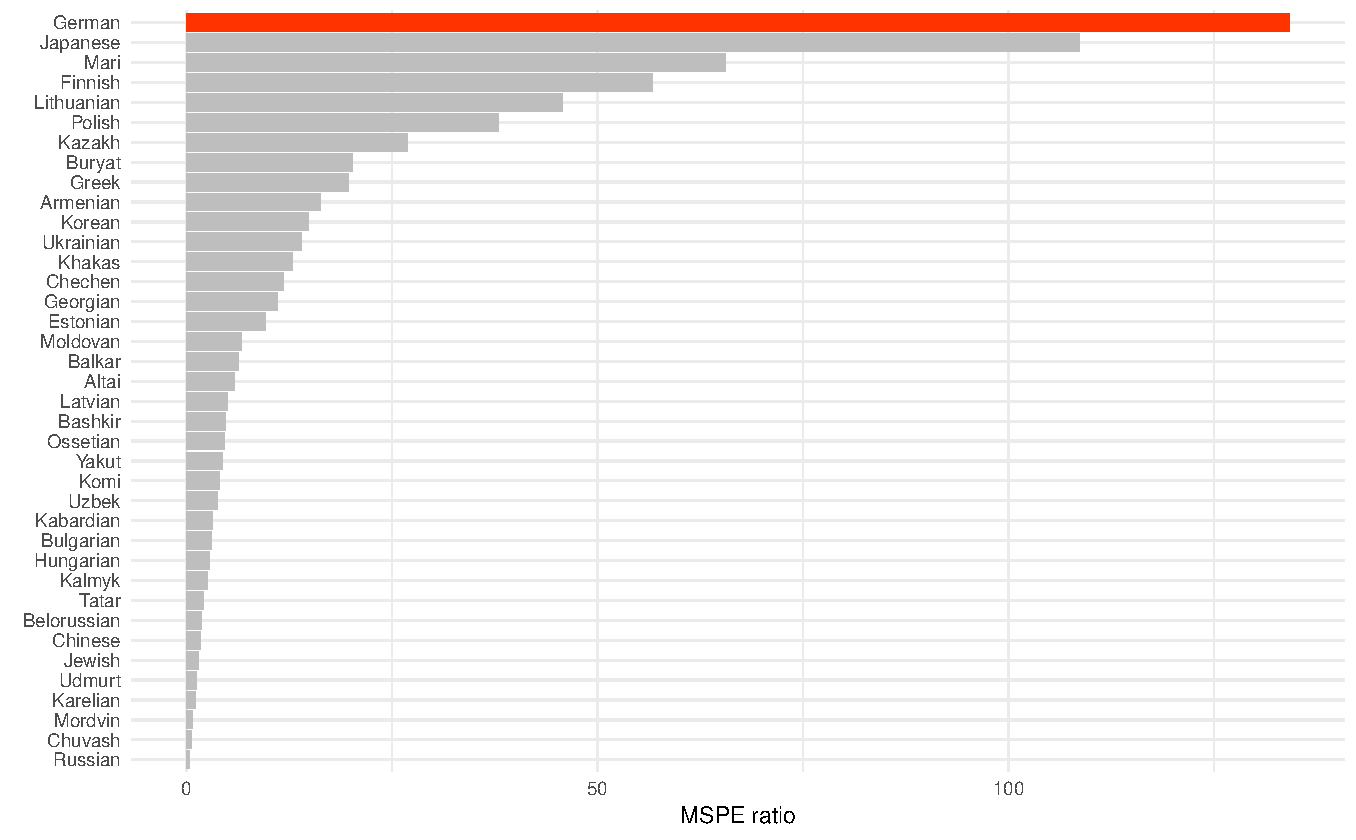
\includegraphics[width=\linewidth]{plots/synthetic_control/ethnicity_imputation/annual/mspe_ratios_imp_date.pdf}
\label{fig:sc_mspe_ratios_all}
\end{subfigure}
\begin{subfigure}{\textwidth}
\caption{Only the period from 1933 to 1939 in the numerator}
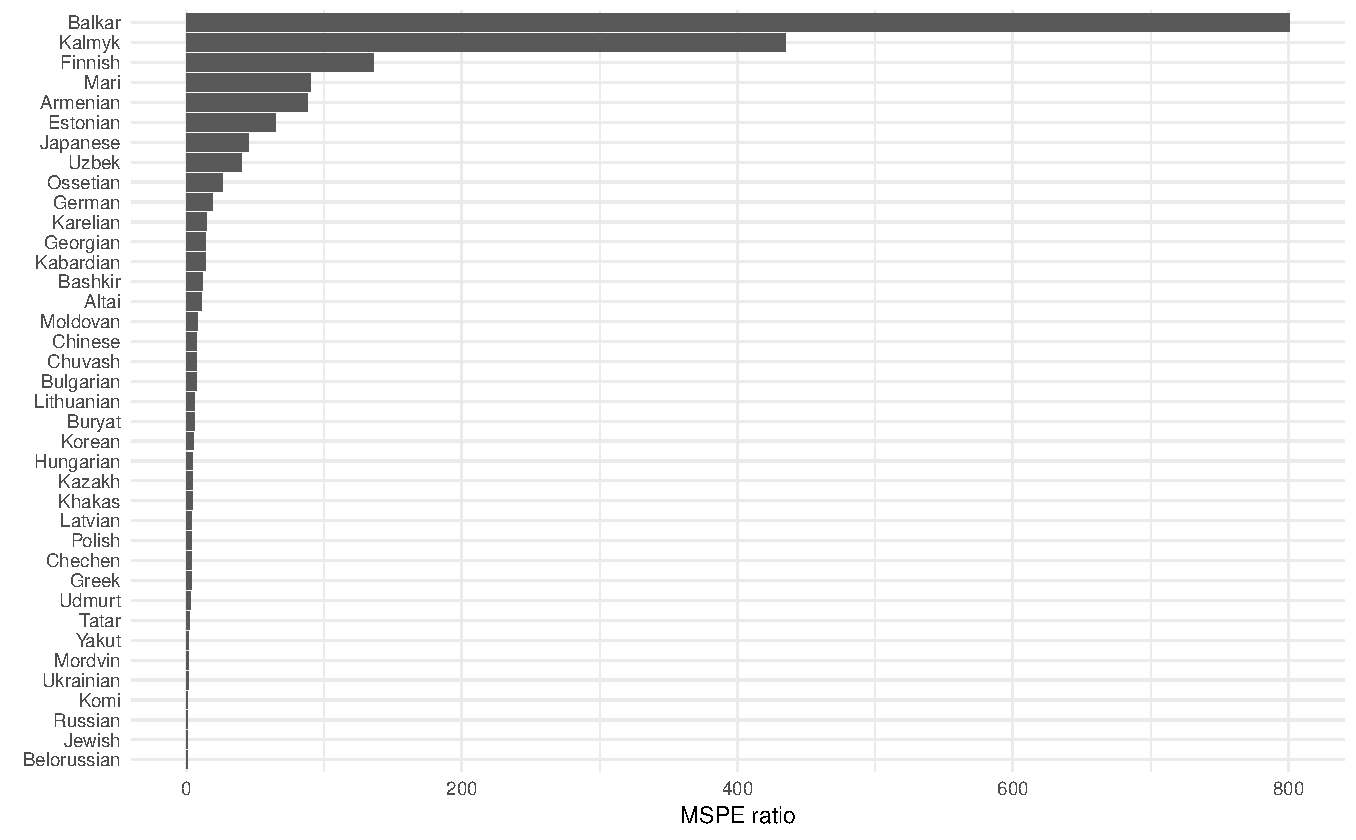
\includegraphics[width=\linewidth]{plots/synthetic_control/ethnicity_imputation/annual/mspe_ratios_imp_date_until_1939.pdf}
%Ethnic groups with pre-treatment MSPE higher than 5 times the MSPE of Germany excluded
\label{fig:sc_mspe_ratios_until_1939}
\end{subfigure}
\label{fig:sc_mspe_ratios}
\end{figure}


%This is shown in  the figure \ref{fig_sc_mspe_hist}


\section{Robustness Checks} \label{subsec:robust_checks}
\subsection{Difference-in-differences}
First, we consider if the presence of ethnicity-specific time trends affects the results.
%As we explained in the methodology section, 
% the ethnicity-specific time trends allows us. 
The estimates regressions with quadratic (default), linear, and no time trends are  plotted in the figure \ref{fig:did_robustness_time_trends} in the appendix. The coefficients for the model with no ethnicity-specific time trends are somewhat lower for the baseline model and the estimates for linear time trends are lower still. Nonetheless, the main general pattern is preserved in all specifications.

Second, we test the sensitivity of results to different adjustments of ethnicity imputation. 
As we explain in the subsection \ref{subsubsec:pred_adj}, the adjustments were applied in order to correct for the unbalanced accuracy in prediction of our Naive Bayes classifier across ethnic groups. The results from fitting our default specification to data with different adjustments are shown in the figure \ref{fig:did_robustness_pred_adj}.
We see that the estimates for the full matrix (used by default) and the parsimonious adjustment are virtually the same. When no adjustment is applied, the coefficients even get slightly larger. 
\subsection{Synthetic Control Method}
 We construct a synthetic control  using mean of the outcome in the pre-1933 period instead of including outcome for every year as we did in our baseline model. This increases the importance of the time-invariant covariates (population, urbanization rate, and linguistic similarity) that are also included as predictors.
\begin{table}[!h]

\caption{\label{tab:sc_predictor_means_robustness}Pre-treatment Predictor Means}
\centering
\begin{threeparttable}
\fontsize{10}{12}\selectfont
\begin{tabular}{lrrrr}
\toprule
\multicolumn{1}{c}{ } & \multicolumn{2}{c}{German minority} \\
\cmidrule(l{2pt}r{2pt}){2-3}
Variable & Actual & Synthetic & Mean of all ethnicities & $V$ weights\\
\midrule
Log(1 + arrests) & 5.59 & 5.48 & 3.649 & 0.15\\
Total population & 1 238 549.00 & 1 747 879.23 & 3 681 250.421 & 0.84\\
Urbanization rate & 14.92 & 21.56 & 17.844 & 0.00\\
Ling. similarity to Russian & 1.00 & 1.16 & 0.763 & 0.00\\
\bottomrule
\end{tabular}
\begin{tablenotes}
\item \textit{Note: } 
\item Log(1 + arrests) is averaged over the pre-treatment period (1921-1932). All other predictor are time-invariant. Total population and urbanization rate are taken from 1926 Soviet census.
\end{tablenotes}
\end{threeparttable}
\end{table}

Recall that the predictors weights $V$ are chosen to minimize pre-treatment MSPE. We can thus infer from the calculated  weights $V$ (provided in the table \ref{tab:sc_predictor_means_robustness})  that neither urbanization rate nor linguistic similarity to Russian are good predictors of pre-1933 repressions. 
%Total population seems to be the most powerful predictor.
Therefore the $W$-weights of ethnic groups in the synthetic control are chosen to mainly match the German minority on population and the mean of $\log\left(1 + \text{arrests}\right)$. 
 The calculated $W$-weights  are shown in the table \ref{tab:sc_weights_robustness}. We see that Tatar and Polish minorities are now contributing with the largest share to the synthetic control. 

\begin{table}[t]

\caption{\label{tab:sc_weights}Synthetic German minority weights}
\centering
\begin{tabular}{lr}
\toprule
Ethnic group & $W$-Weight\\
\midrule
Tatar & 0.49\\
Polish & 0.39\\
Korean & 0.12\\
\bottomrule
\end{tabular}
\end{table}

When we compare the gaps between synthetic control and actual value (figure \ref{fig:sc_placebo_gaps_robustness}) with our baseline model, we notice three main differences. First, pre-treatment fit for Germany is substantially worse which is the the cost
assigning greater importance to other covariates by  using only the pre-treatment mean of the outcome. Second, the gap for the years 1933-1939 is slightly smaller. Finally, there is large drop in the estimated effect in the year 1944. This most likely a consequence of the sharp increase in repressions of Tatars in 1944 following their mass deportations from Crimea that year. 
%contributing to the 
Nonetheless, both our baseline model and its robustness check otherwise follow very similar trends.
The $p$-value of the effect for the whole period 1933-1960  is again 1/38 ($\approx 0.026$). However if we consider only the time window of  1933-1939, the 
$p$-value increases to 1/19 ($\approx 0.105$). The MSPE ratios for all ethnic groups based on which the $p$-values were calculated are provided in the figure \ref{fig:sc_mspe_ratios_robustness}.